\documentclass[12pt,doublespace]{report}
\usepackage[margin=1in]{geometry}
\usepackage{multicol}
\usepackage{caption}
\usepackage{subcaption}
\usepackage{graphicx}
\usepackage{float}
\usepackage{epstopdf}
\usepackage{setspace}
\usepackage{abstract}
%\usepackage{grffile}
\usepackage{pdfpages}
\usepackage{lscape}
\usepackage{authblk}

\usepackage{fancyhdr}
	\pagestyle{fancy}
	\fancyhead[L]{\today}
	\fancyfoot{}
	\fancyhead[C]{OCE 495 Section 2}
	\fancyhead[R]{\thepage}


\title{\vspace{-5mm}
	\fontsize{20pt}{10pt}\selectfont
	Embedded Wireless Sensor Design for Long Term Structural Health Monitoring
}
		
\author[2]{Christopher Bessin}	
\author[1]{Patrick Blum}
\author[1]{Matthew P. Iannucci}
\author[1]{Jordan T. Kirby}
\author[1]{Zachary McIntosh}
\author[2]{Elizabeth L. Paul}
\author[1]{Michael A. Regan}
\author[2]{Justin W. Skenyon}
\author[1]{Charles J. Wesley}
\author[1]{Samuel D. Wiley}

\affil[1]{Finite Element Modelling}
\affil[2]{Instrumentation Development}
\date{\normalsize\vspace{-3mm}\today}



\begin{document}
\maketitle

\textit{I have read this paper in its entirety and approve it for submission.}
\vspace{1.5cm}
\begin{flushleft}

\noindent\begin{tabular}{ll}
\makebox[2.5in]{\hrulefill} & \makebox[2.5in]{\hrulefill}\\
Christopher Bessin & Date\\[4ex]% adds space between the two sets of signatures
\makebox[2.5in]{\hrulefill} & \makebox[2.5in]{\hrulefill}\\
Patrick Blum & Date\\[4ex]
\makebox[2.5in]{\hrulefill} & \makebox[2.5in]{\hrulefill}\\
Matthew P. Iannucci & Date\\[4ex]
\makebox[2.5in]{\hrulefill} & \makebox[2.5in]{\hrulefill}\\
Jordan T. Kirby & Date\\[4ex]
\makebox[2.5in]{\hrulefill} & \makebox[2.5in]{\hrulefill}\\
Zachary McIntosh & Date\\[4ex]
\makebox[2.5in]{\hrulefill} & \makebox[2.5in]{\hrulefill}\\
Elizabeth L. Paul & Date\\[4ex]
\makebox[2.5in]{\hrulefill} & \makebox[2.5in]{\hrulefill}\\
Michael A. Regan & Date\\[4ex]
\makebox[2.5in]{\hrulefill} & \makebox[2.5in]{\hrulefill}\\
Justin W. Skenyon & Date\\[4ex]
\makebox[2.5in]{\hrulefill} & \makebox[2.5in]{\hrulefill}\\
Charles J. Wesley & Date\\[4ex]
\makebox[2.5in]{\hrulefill} & \makebox[2.5in]{\hrulefill}\\
Samuel D. Wiley & Date\\[4ex]
\end{tabular}
\end{flushleft}

\begin{abstract}
Structural health monitoring is the process of continuously
monitoring the vibrations of a structure and analyzing long term
changes in the natural frequency to detect internal or external
damage and its location, type, and severity. By the completion of
this project, multiple sensor packages intended to monitor the
structural health of the Claiborne Pell Newport Bridge will be
designed, built, and installed. In the initial phase of this
project, the bridge was considered to be a simply supported
beam. Sensor packages consisting of an accelerometer and a
strain gauge, with supporting microprocessor and analogue
to digital converter were secured to both an I-beam and
angle beam to measure vibration data. These beams were
chosen as preliminary representations of the bridge as
they will have comparable modal responses. A finite element model
(FEM) was produced to calculate the modal responses of the beams,
which were used to determine the optimal locations for the sensor
packages. The FEM analyses were verified with analytical
solutions and experimental data, confirming the natural
frequencies for the I-beam and the angle beam. The sensor
packages were installed on the angle beam and modes 1-5 were
detected and matched the theoretical analyses and FEM. Sensor
packages similar to this are currently availabe, however, no
packages offer wireless communication capability, power
independence, and a minimal power draw at a reasonable
price. In the second phase of this project the sensor
packages will be modified for installation on the Pell
Newport Bridge.

\end{abstract}
\section*{Acknowledgments}
The group would like to thank the following people for their continued support throughout the duration of this project:

\begin{itemize}
\item Dr. Harold "Bud" Vincent II and Dr. San-Lou Hu for being our faculty advisors.
\item Manoj Menon - Ocean Engineering Graduate student who aided greatly in the finite element modeling portion of this project.
\item Eric Offenburg - Contact at Rhode Island Bridge and Turnpike Authority.
\end{itemize}
\tableofcontents
\listoffigures
\listoftables
\chapter{Introduction}
\indent Effort has been made in recent years toward structural health monitoring development as evaluating the fatigue of existing infrastructures will improve will safety. According to the National Bridge Inventory, $90\%$ of all daily traffic utilizes a state or federal owned bridge so the need of ensuring that these structures are properly maintained and rebuilt when necessary is imperative \cite{RobertS.Kirk:2007}. \\
\indent In the 1950s the Interstate Highway System inspired a building surge that resulted in what are now referred to as the baby boomer bridges. Unfortunately, these bridges were built to last for 50 years as it was anticipated that with the development of materials and technology these bridges would be obsolete in that time \cite{AmericanAssociationofStateHighwayandTransportationOfficials:2008}. An unforeseen economic hardship both in the country’s compromised financial situation and in dramatic construction cost increase has made this replacement process near impossible. In recent years immediate closures prompted by large scale structural hazards in the form of cracks or corrosion lead to huge displacements of traffic \cite{AmericanAssociationofStateHighwayandTransportationOfficials:2008}. \\
\indent Structural health monitoring can detect internal damage by sensing the resulting vibration change the bridge experiences. The source of this damage can be attributed to long term fatigue from aging, and short term events such as weather, flooding, or traffic. By interpreting these vibration changes the location and extent of damage can be potentially deciphered. Without visual inspection of the bridge large-scale failure can be evaded, making the bridges safer and avoiding immediate closures. \\
\indent In designing and prototyping a structural health monitoring sensory package for the Caliborne Pell Newport Bridge finite element modeling, confirmed by analytical solution, need to be explored. The foremost concern of the structural health of the Pell Bridge is to ensure structural integrity and guarantee the safety of the travelers. The recent collapse of the I-35W Bridge in Minneapolis and the quarter of bridges in the United Stated that were deemed structurally deficient according at a recent structural survey, has provoked the development of structural health monitoring systems and the need for standards to be set. If a structure is continuously monitored then damage can be detected by the changes reflected in the data. Accurate sensory systems can detect that damage has occurred, located the damage, and evaluate the extent of the damage. With the widespread adaptation of monitoring systems data can be compiled and used to produce standards. 


\section{Objectives}
\subsection{Phase One (Fall 2013)}
\indent To produce FEMs of the simply supported beams which concur with analytical solutions and indicate the modal response. Design and produce a sensory package to collect accurate vibration data. Compare experimental data with FEM. \\
\subsection{Phase Two (Spring 2014)}
\indent To modify the sensory package design to be installed on the Pell Bridge by being power independent and wireless communication capabilities. Model the Pell Newport Bridge to predict modal frequency.\\
\section{Layout} %FIX ME!!!!!!!!!!!!!!!!
This report will discuss the planning process of designing a sensor package intended to evaluate vibration on the Pell Bridge. As this is a two-semester project the preliminary assembly of the package was simplified to evaluate vibrations of a 6.8 meter angle beam. A finite element model was produced of this angle beam to provide information on the modes of vibration and natural frequency. \\
\indent The extension of this project will include modifying the sensor package to be implemented on the Newport Bridge. A Finite Element Modeling will be drawn in Abaqus to indicate where we should install the sensors and what the natural frequency of the bridge will approximately be. \\
\indent Chapter 3 will explains the finite element model of the angle beam and what parameters were used to describe the material. To prove that the finite element model was reflecting accurate natural frequencies and modes of vibration, these model was verified with the analytical solution for the beam, this evaluation is described in detail in chapter 3. \\
\indent Choosing the appropriate, cooperating instrumentation is integral to producing a sensor package that will accurately monitor the bridge. Chapter 4 of this report will present the instrumentation chosen and why. \\
\indent After the preliminary package was assembled data was collected and processed for the 6.8 meter angle beam. The collection process and processing details are discussed in chapter 5 and 6. \\ 
\indent As this sensor package is intend for the Pell Newport Bridge necessary modifications were researched for remote installation. Power independence is required along with wireless communication capabilities. The intended modifications are discussed in chapter 7. 


\chapter{Instrumentation Package}
\input{INSTRUMENTATION_INTRO}
% % % % % % % % % %MATT'S SECTION
\section{Microprocessor}
\label{sec:uProcessor}
\indent At the core of the sensor package is the microprocessor. The
microprocessor served as the data collection and distribution
device. The module received data from the peripheral devices and
either stored the data for further analysis or distributed it in
some manner. However, because of both the project requirements
and the diversity of the sensors, choosing the right
microprocessor meant looking closely at all of the requirements
for operation. These requirements may be seen below. 
\subsection{Necessary Specifications}
\subsubsection{Power Consumption}

\indent Though power was not a focus of this semester, the
microprocessor of choice was to be used through the next semester
as well. This means the module of choice should be low power and
made for embedded applications. 

\subsubsection{Timing Accuracy and Synchronization}

\indent Another important area to consider is the ability to time
synchronize with a central clock. This was also not a concern for
the prototyping stage this semester but the same board will be used
for the coming semester. In some way it must be feasible for the
computer chosen to communicate with a clock source and
synchronize itself. This could mean communicating with an
external GPS module or with a remote NTP server. 
\subsubsection{Sampling Frequency}

The microprocessor must be able to sample data from peripheral sensors at a rate fast enough to avoid aliasing data. Analysis from the Finite Element Modeling team was used to decide on this parameter

\subsubsection{Input Output Capabilities}

In order for the processor to collect and relay data from many
different sensors, there are strict input output needs. To
communicate with the Analog to Digital Converter (ADC), the
computer needs to have an Inter-Integrated Circuit ($I_2C$) bus.
Two Universal Asynchronous Receiver/Transmitter (UART) buses are
needed to communicate with the GPS module and a wireless
transmitter that has not been determined yet.

\subsubsection{Data Logging}

For testing, the ability to store data to a log file instead of
exporting via wireless was desired. This allowed testing of the
prototype without the use of wireless communications. The data
could be collected and simply stored for later analysis. 


\subsubsection{Software Development}

The platform chosen should a reasonably tested development
environment and SDK. The platform chosen should have a compiler
that makes use of popular languages. It should also be clear, if
more than one language may be used, what the advantages and
disadvantages of each approach would be. For instance, compiling
an executable vs executing a python script. 

\subsection{Platform Options}

\subsubsection{Microprocessor Comparison Table}
\begin{table}
\centering
\begin{tabular}{|l| p{3cm} | p{3cm} |}
\hline
\textbf{Microprocessor:} & BeagleBone Black 
%	\begin{figure}
\includegraphics[scale = 0.25]{BeagleBoneBlack_Image.jpg}
%	\end{figure}
& Netburner MOD5270
%	\begin{figure}
\includegraphics[scale = 0.25]{Netburner_MOD5270_Image.jpg}
%	\end{figure}
\\
\hline
\textbf{Clock Rate:}		&1GHz ARM Cortex-A8& 145.7MHz 
Freescale ColdFire 5270 \\
\hline
\textbf{I/O Pins:}		& 65  &46\\
\hline
\textbf{Power Consumption:}&	1.05-2.3 W @ 5V	& 1.65 W @ 3.3V	\\
\hline
\textbf{Data Storage:}	&			microSD		&	microSD	\\
\hline
\textbf{Supported Communications:}&	I$^2$C, SPI, 3 Serial 
Ports		&I$^2$C, QSPI, 3 Serial Ports		\\
\hline
\textbf{Software Development}&Python,C/C$^{++}$&C/C$^{++}$\\
\hline
\end{tabular}
\caption{\textit{Comparison table of two microprocessors that 
were looked into for the embedded sensor package}}
\label{tab:uProcOptions}
\end{table}

\subsubsection{BeagleBone Black}
\label{subsec:BeagleBoneBlack}
\indent The BeagleBone Black is single board computer (SBC) that
runs a Linux operating system (Angstrom). The board is powered by a
TI AM3358 Sitara ARM Cortex-A8 Microprocessor. The core is 32 bit,
and can reach up to 1 GHz clock speeds. The board comes with a
plethora of pins. Included are two $I_2C$ buses, four UART
ports, and over 60 GPIO pins. There are also ground, 3.3V, and
5V pins to drive peripheral devices. \\

\indent The board runs full blown Linux and root access is
available. This means that development is possible with a variety
of languages from C++ to Java-script More importantly, there are
third party API (Application Programming Interface) libraries for
the all of the board's input and output written for both Python
and Java-script Both are high level languages and allow for
efficient code development and quicker testing of hardware
development. 

\subsubsection{Netburner MOD5270}
\label{subsec:MOD5270}
\indent The Netburner MOD5270 is a powerful embedded
micro-controller The drawing feature of this board is the inclusion
of a real time clock and its Real Time Operating System. It brings
predictable multitasking and timing. Furthermore, there is an
on-board SD card slot that can be used for real time data
logging. The processor is a 32-bit Freescale ColdFire 5270
running at 145.7 MHz. The on-board Direct Memory Access (DMA)
timers are optimal for timing the application and
synchronizing data transfers. There are two UARTs and an
$I_2C$ bus to go along with various General Purpose
Input/Output (GPIO) pins, including interrupt enabled pins
for external triggering if necessary. \\

\indent The board has a C++/C cross compiler. The System Development
Knowledge (SDK) is well documented and there are many examples for
various applications. The Netburner does not run a full operation
system. Instead, it runs a Real Time Operating System which
handle multitasking with priority levels and cycling. This is
much preferred to a full operating system for an embedded system
as it makes timing more precise and the processor more
efficient. However, the downside to the low level nature of
the board is the development difficulty. The development is
more difficult and takes more time and precision to
perfect. It is also more difficult to modify than a higher
level program running atop a traditional OS layer as seen
in the BeagleBone Black.

\subsection{Platform Decision}

The BeagleBone Black was the single board computer chosen for the
system. The system clock is fast enough to handle data at a rate of
1 kHz, the maximum sampling rate that was used for data
collection. Also, there are four serial buses, so the board was
able to receive data from the external GPS receiver module.
Importantly, the board allowed for fast development with the
Analog to Digital converter chosen. Development would have
been much slower if a different board had been chosen. The
board was chosen because of its ability to satisfy all of the
requirements for the microprocessor while allowing for
dynamic testing throughout the prototyping stage. 

%\section{Software Design}
The software design controls the timing and data collection for the
package. The software structure is simple, yet crucial. In order to
keep the data collected by the package relevant, the software
logic and timing needed to be in order. \\

The first state in the software design is the initialization state.
Here, the analog to digital converter was initialized through I2C
communication. The handle of the analog to digital communication
object was saved for later use in the next state. Once the
initialization state was finished, the application proceeded
to the sampling state.\\

In this application, 200 Hz was decided to be the target sampling
rate. The program waited for an interrupt then the system time 
has reached a user-defined time. This is important because every 
sensor package waited for the same time and they sampled  
at the same instant (accurate to a millisecond). When the signal was received, 
the application proceeded to collect data from the peripheral sensors. For
each sample during the sampling duration, data was collected
from the ADC via I2C. The data structure was appended over the sampling entire
sampling period and passed as a return from the state.
Once the sampling duration was over, the data logging
state was begun. \\

The data logging state received the data structure created in the
previous sampling state. This data was then sorted and written to a
standard comma delimited text file. The file stream was closed
once all of the data had been written and the program finishes. A
simple block diagram of this flow can be seen in Figure
\ref{fig:PRO_SoftFlow}.

\begin{figure}[H]
\centering
\includegraphics[width = 4in]{"Software flow"}
\caption{\textit{Software flow of the sensor package}}
\label{fig:PRO_SoftFlow}
\end{figure}
%\section{Analog-to-Digital Data Converter}
\subsubsection{Necessary Specifications}
\label{sec:ADC_Parameters}
\indent The BeagleBone Black microcontroller features an on board 12-bit analog-to-digital converter (ADC). From literature, the lowest acceptable
effective resolution that an ADC being used for SHM may have is 16 bits\cite{Cunha_Caetano} \cite{JangSWMWSS}. It was determined that the need for an
external ADC was present. The parameters of the external ADC needed were as follows:
\begin{itemize}
\item High Resolution
\item Appropriate Sampling Frequency
\item Low Power Consumption 
\item Support for Multiple Input Channels
\item Communicate via Serial Interface
\end{itemize}
\paragraph{Resolution}
\label{sec:adc_res}
\indent Resolution is defined as the number of bits that an analog signal is mapped to after being converted\cite{MusaJouaneh:2013}. Using the chart in
Figure \ref{fig:ADC_Comp_Chart}, it was evident that in order to achieve high resolution data that a Delta-Sigma ($\Delta\Sigma$) ADC needed to be used.\\
\indent As previously stated, the minimum resolution required for this sensor package was 16-bits. The voltage resolution can be found using Equation
\ref{eqn:Resolution}:
\begin{equation}
\label{eqn:Resolution}
V_{Res} = \frac{V_{Range}}{2^{n}}
\end{equation}
Assuming $V_{Range}=3.3V$, $n=16$ bits then $V_{Res}$ is approximately $50.35\mu V/$division. 

\begin{figure}[H]
\centering
\includegraphics[scale=1]{KIRBY_Images/ADC_Comp_Chart.jpg}
\caption{\textit{Chart displaying the classifications of different ADC architectures \cite{WaltKester:2005}}}
\label{fig:ADC_Comp_Chart}
\end{figure}
%
\paragraph{Sampling Rate}		%EDIT THIS SECTION
\label{sec:adc_fin}
\indent The Nyquist-Shannon Sampling Criterion states that data must be sampled at a minimum of twice the expected frequencies being measured
\cite{MusaJouaneh:2013}. The accelerometer that was chosen for the preliminary lab experiments has a bandwidth of $500 Hz$, therefore the ADC must be able
to sample a minimum of $1kHz$. However, since frequencies expected from the lab testing are in the range of $0-60Hz$, the sampling frequency of the ADC
does not necessarily need to be so high. %Must reference source that states expected natural frequencies of bridges
%
\paragraph{Power Consumption}
\label{sec:adc_power_cons.}
\indent Since the nature of this sensor package was to be a wireless sensor, it was assumed that all power used by the sensor package would be generated
using alternative energy. With this in mind, components used on board the sensor package have as little current draw as possible.
%
\paragraph{Input Channels}
\label{sec:adc_in_ch_num}
\indent One important, but almost overlooked, characteristic of the ADC was the ability to support multiple input channels simultaneously. The ADC needed
to be able to read three channels from an accelerometer and at least two channels from a strain gauge. For prototyping purposes, it is typically difficult
to find ADC's with more than 4 inputs; most come in as surface mount components and require a printed circuit board. It became evident as the project progressed that each input device would need a dedicated ADC due to the multiplexer switching time of multi-channel ADC units. 
It was decided to address this problem by interfacing four ADC units simultaneously on a serial communication bus.
Subsection \ref{sec:adc_comm} discusses this in further detail.
It should also be noted that the inputs of the ADC were configured for differential measurements.
This gives the ability to compare the sensor data to a noise reference, and thus make reducing data filtering during processing. 
%
\paragraph{Communication}
\label{sec:adc_comm}
\indent As shown in Table \ref{tab:uProcOptions}, the BeagleBone Black supports multiple communication protocols, include but not limited to, SPI and
I$^{2}$C. The communication from the ADC to the main micro-controller was decided to be either  4-wire SPI or I$^{2}$C. The ADC will be the slave to the
micro-controller. A con using SPI as the communication method is that for each slave device in the communication loop, there must be a dedicated Slave
Select (SS) line. This puts a limitation on how many ADC's can be used in each sensor package. However, I$^{2}$C utilizes a central bus and 7 bit unique
addresses for slave selection.

\subsubsection{Analog-to-Digital Converter Selection}
\indent When searching for ADC's that fit the parameters set in Section \ref{sec:ADC_Parameters}, three devices were investigated; the TI ADS1211, TI
ADS1115 and the TI ADS1113. The devices are summarized in Table \ref{tab:ADC_Compare} and explained in detail below.

\begin{table}[H]
\begin{center}
\begin{tabular}{|p{3cm}| p{3cm} | p{3cm} | p{3cm}|}
\hline
&\multicolumn{3}{c|}{\textbf{Analog-Digital Converter}}\\
\hline
\textbf{Parameter} & ADS1211 & ADS1115 & ADS1113\\
\hline
Package &\includegraphics[width = 2.5cm]{KIRBY_Images/oldadc}
&
\includegraphics[width = 2.5cm]{KIRBY_Images/ads1115} & \includegraphics[width = 2.5cm]{KIRBY_Images/ADS1113_msop10}\\
\hline
Resolution: & 24 bits & 16 bits & 16 bits\\
\hline
Supported Communications:&	 SPI & I$^2$C & I$^2$C \\
\hline
Power Consumption:&	5mW @ 5V	& 0.66 mW @ 3.3V & 0.66 mW @ 3.3V\\
\hline
Number of Inputs: & 4 & 4 & 1\\
\hline

\end{tabular}
\caption{\textit{Comparison table of the ADS1211, ADS1115 and ADS1113 ADC devices}}
\label{tab:ADC_Compare}
\end{center}
\end{table}


\paragraph{TI ADS1211}
\label{sec:ADC_ADS1211}
\indent The Texas Instruments ADS1211 24-Bit $\Delta \Sigma$ analog to digital converter features 20 effective bits of resolution at $1kHz$ under ideal
conditions; however that would be contingent upon the ability to design an ideal printed ciruit board (PCB) for the converter. Between 16 and 18 bits of
resolution are realistic for the initial prototype of the sensor package. By utilizing an internal 4-to-1 multiplexer, four input channels are available
to use. Recall that Section \ref{sec:adc_in_ch_num} requires at least five input channels, the ADS1211 falls short here. As a solution two ADC's would
be used, making it possible to read two strain gauges per sensor package as opposed to one. The ADS1211 datasheet provides information on synchronizing
multiple ADC's together. The converter draws approximately $10mA$ under typical working conditions. The converter utilizes the SPI protocol that is
supported by the BeagleBone Black.\\
\indent The ADS1211 was purchased and interfaced; however due to the complex circuitry that was required by the device, a month passed before the chip was
tested. The converter functioned correctly for approximately ten minutes and then stopped transmitting data. 
\paragraph{TI ADS1115}
\label{sec:ADC_ADS1115}
\indent The Texas Instruments ADS1115 16-Bit analog to digital converter is of the same architecture as the ADS1211 ($\Delta \Sigma$). The chip also
features a multiplexer that allows up to 4 single ended or 2 differential inputs. The sampling frequency of the ADC is programmable from 8Hz to 860Hz, and
includes an internal oscillator. The average current draw for the ADS1115 is approximately $150\mu A$. There are two notable differences between the
ADS1115 and the ADS1211 ADCs. First, the ADS1115 communicates via the I$^{2}$C communication protocol. The ADS1115 has four unique I$^{2}$C addresses;
making it possible to have 16 single-ended inputs on one communication bus. Also, the chip was available pre-mounted on a PCB with all the necessary
supporting hardware; thus eliminating the possibility of incorrectly wiring up the circuit. 
\paragraph{TI ADS1113}
\label{sec:ADC_ADS1113}
\indent The TI ADS1113 is within the same family as the ADS1115, only differing in the number of input channels and not having internal programmable gain amplifiers and comparator.
Like the ADS1115, four ADS1113 units can be on the same I$^{2}$C bus, can also run in continuous sampling mode, and also shares the same library of functions as the ADS1115.
Since the ADS1113 does not multiplex its inputs, there is no loss of data between switching.
The dissadvantage to the ADS1113 is that it is only available as a surface mount chip (MSOP-10 package); thus requiring more circuitry on the printed circuit board.

\paragraph{ADC Impedance Matching}
\label{sec:ADC_Impedance_Issues}
Preliminary lab tests were performed using a micro-controller with 12-bit ADC to collect data for analysis.
The time series that was returned did not accurately represent the data present, as verified with an oscilloscope.
It was determined that this was due to a difference in impedances between the accelerometer and the ADC.
The solution was to construct an op-amp circuit to match the impedances of the accelerometer and the micro-controller inputs.
It was initially believed that the internal programmable gain amplifiers (PGA) of the ADS1115 would avoid such issues in impedance matching.
However, after further research it was discovered that this assumption was incorrect.


\paragraph{ADC Final Selection}
\indent Based on the comparison of the ADS1211, ADS1115 and ADS1113 ADC's, the ADS1115 was chosen for the preliminary package to test code before the printed circuit board was designed.
For the final package, four ADS1113 ADC units were integrated into the PCB design as discussed in Section \ref{sec:ADC_Impedance_Matching}. 


\section{Sensors}
% % % % % % % % %SAM & ZAC
\subsection{Accelerometer}
\indent Accelerometers were implemented in this package to determine the frequencies at which the element vibrates at. For lab testing, the desired data was the modal shapes of an L beam. The use of accelerometers for structural health monitoring is becoming common practice in smart bridges such as the new I-35W bridge in Minneapolis where periodic modal studies are performed\cite{Kistler}.

\subsection{Accelerometer Parameters}
\indent When choosing the correct accelerometer to be implemented in the sensor package, the following parameters were deciding factors:
\begin{itemize}
\item Number of Axes
\item Dynamic Range
\item Type of Mount
\item Analog vs Digital Output
\item Bandwidth
\item Power Consumption
\end{itemize}

\subsubsection{Number of Axes}
\indent The number of axes is regarded as how many directions that acceleration may be measured. Typically accelerometers have at least two axis. For the purposes of the sensor package, three axis were needed.
\subsubsection{Dynamic Range}
\indent The main limiting factor for determining the proper accelerometer was the dynamic range (DR).  This refers to the range of accelerations that the sensor is capable of measuring. For a 3g accelerometer, the device can measure accelerations up to $3*9.81m/s^{2})$ or$ 29.43 m/s^{2}$.  The value of the dynamic range is found on its corresponding data sheet.  To determine the appropriate accelerometer, the proper DR had to be determined.  This value is a dependent upon three parameters.  The equation for the dynamic range , Equation \ref{eqn:Acc_Accel} below, is dependent on the frequency being sought after and the resulting amplitude.  This equation is derived from the position function, Equation \ref{eqn:Acc_Pos};  
%Latex Code
\begin{equation}
u = Ae^{j\omega t}
\label{eqn:Acc_Pos}
\end{equation}
\begin{equation}
\dot{u} = Aj\omega e^{j\omega t}
\label{eqn:Acc_Vel}
\end{equation}
\begin{equation}
\ddot{u} = -A\omega^{2}e^{j\omega t}
\label{eqn:Acc_Accel}
\end{equation}

\noindent where $u$ is the position, $\ddot{u}$ is acceleration (or in this case the DR), \textit{A} is the displacement, $\omega$ is the measured frequency in radians, and \textit{f} is the frequency in Hertz.  This equation allows one to calculate the allowed maximum displacement before reliable data cannot be measured.  Since the frequency value of the acceleration function is squared, a change in frequency will cause a dramatic change in the maximum allowed amplitude.  Using a maximum frequency of 77.5 Hz (determined analytically by the FEM team) and a 1.5 Hz frequency (a rough representative of the Newport Bridge), the maximum displacement of a structure before unreliable data acquisition occurs was calculated for every accelerometer that was considered.  These values are shown in Table \ref{Acc_Comp_Table}.

\subsubsection{Type of Mount}
\indent Accelerometers can be mounted to a circuit board in one of two manors: through-hole mounting or surface mounting.  An accelerometer with dual inline package (DIP) header pins can be placed directly into a breadboard for prototyping; whereas a surface mount accelerometer needs to be specially soldered to a PCB.
\subsubsection{Analog vs Digital Output}
\indent The difference between an analog and digital accelerometer is how the output data is processed.  Analog accelerometers output a frequency that is proportional to acceleration whereas digital accelerometers output a square wave of a certain frequency.  The amount of time that the wave is high is proportional to the amount of acceleration \cite{DimensionEngineering}. 
\subsubsection{Bandwidth}
\indent The bandwidth is defined as the useful frequency range in which the response falls to -3dB of the nominal value (0 Hz) \cite{MSY.SivaPrasad:2011}.  Therefore, while choosing an accelerometer, the desired frequencies must fall within the bandwidth of the sensor.   
\subsubsection{Power Consumption}
\indent To conserve power, finding an accelerometer with low current draw was essential.  Fortunately most accelerometers require only a small amount of current draw.

\subsection{Accelerometer Selection}
\indent The comparison of the considered accelerometers is tabled below.  Initially, the AXL330 was chosen as the best option compared to the BMA220 and the ADXL362 because it is an analog accelerometer.  This is because it was determined that an analog accelerometer would allow for the easiest time synchronization of data with the other sensors.  However, during laboratory testing data was being clipped.  This data was deemed unreliable because as data is clipped the response becomes a multiple derelict function instead of a single one.  This causes data fitting to appear like a square wave instead of the intended sinusoidal wave.  Therefore the MMA7361L accelerometer was ordered and used it place of the ADXL330.  

\begin{table}[H]
    \begin{tabular}{|p{2.5cm}|p{2.5cm}|p{2.5cm}|p{2.5cm}|p{2.5cm}|p{2.5cm}|}
    \hline
    \textbf{Parameter} & \multicolumn{4}{c|}{\textbf{Accelerometer Model}}& \textbf{Unit} \\
    \hline
            & BMA220 \includegraphics[width = 2.25cm ]{ACC_BMA220}    & ADXL362  \includegraphics[width=2.25cm]{ACC_adxl362}  & ADXL330  \includegraphics[width = 2.25cm ]{ACC_adxl330} & MMA7361L \includegraphics[width = 2.25cm ]{ACC_mma7361l} &  \\ \hline
    Analog/ {Digital}            & Digital                   & Digital            & Analog      & Analog        & ~ \\ \hline
    Dynamic Range              & $\pm$2/4/8/16g            & $\pm$2/4/8g         & $\pm$3g     & $\pm$1.5/6g   & m/s$^2$ \\ \hline
    Maximum Displacement @ 77.5 Hz & 0.083/0.165/ 0.331/0.661   & 0.083/0.165 /0.331   & 0.124       & 0.062/0.248   & mm    \\ \hline
    Maximum Displacement @ 1.5 Hz  & 220.9/441.7/ 883.5/1766.9  & 220.9/441.7/ 883.5   & 331.3       & 165.7/662.6   & mm    \\ \hline
%   \textbf{ Bandwidth}                  & ~                         & ~                   & ~           & ~             & ~     \\ \hline
    Bandwidth: X \& Y-axis               & 32/64/125/ 250/500/1000    & 50/200              & 0.5-1600    & 400           & Hz    \\ \hline
    Bandwidth: Z-Axis                     & 32/64/125/ 250/500/1000   & 50/200              & 0.5-550     & 300           & Hz    \\ \hline
    Current Draw               & 250 @ 3V           	   & 3 @ 2V   		     & 320 @ 3V    & 400 @ 3.3V    & $\mu$A     \\ \hline
    Power Consumption          & 750                       & 6                   & 960         & 1320          & $\mu$W    \\ \hline
    Number of Axes             & 3                         & 3                   & 3           & 3             & ~     \\ \hline
    \end{tabular}
    \caption{\textit{Comparison table of four accelerometers that were possible candidates for the sensor package.}}
\label{Acc_Comp_Table}
\end{table}


\subsection{Strain Gauge}
\indent The deformation and displacement that an object feels under an external force is defined as strain \cite{OmegaEngineeering:2013}. In the applications of engineering and construction the strain of an object, such as a support or beam, is a necessary component to monitoring the structure. To measure the strain of a structure, a strain gauge may be applied. The strain gauge can be a very effective measurement technique for SHM because it has the ability to measure the compression and expansion within the members of the structure. The strain values measured on the structure can be used to state the stress within the material to monitor and predict the safety of the structure. The change in capacitance, inductance or resistance is proportional to the strain experienced by the sensor. The strain sensitivity or gauge factor is a dimensionless figure that represents the tolerance of the gauges . It allows for the gauge to have minimal imprecision for changes in temperature. Equation \ref{eqn:Strain_GaugeFactor} shows the calculation of the gauge factor (GF) for a strain gauge

\begin{equation}
GF = \frac{\Delta R / R}{\epsilon} 
\label{eqn:Strain_GaugeFactor}
\end{equation}
\indent Where $\epsilon$ is the lateral or longitudinal strain; defined by \ref{eqn:Strain_StrainEqn}.

\begin{equation}
\epsilon = \frac{\Delta L}{L}
\label{eqn:Strain_StrainEqn}
\end{equation} 

\indent Ideally strain would only change due to a change to the surface the sensor is attached to. However, temperatures, material properties, the bonding adhesive and the stability of the metal all affect the detected resistance. So when selecting a strain gage one must be thorough in understanding the conditions the gage may be under during use. Because material properties are not the same in each direction, only knowing axial strain is not enough. We also need Poisson Strain and Shearing Strain to calculate the Principal Strain. Poisson Strain is both the thinning and widening of the beam, as well as the elongation that the beam may feel under strain. Shearing Strain is the angular distortion of the beam, or the angle of rotation or twist due to shear stress. Generally, to calculate the Principal Strains the largest normal strain is of most interest. This can be found by taking the derivative of $\epsilon X$ or $\epsilon Y$ with respect to $\theta$ and equating it to zero. This gives the principal rotation angle, $\theta p$, this will help produce the principal Strains (max and min); as seen in Equations \ref{eqn:Strain_Ep} - \ref{eqn:Strain_Theta}
\begin{equation}
\epsilon_{p,q} = \frac{1}{2}\biggl[\epsilon_{1} + \epsilon_{3} \pm \sqrt{(\epsilon_{1}-\epsilon_{3})^{2}+(2\epsilon_{2}-\epsilon_{1}-\epsilon_{3})^{2}}\biggr]
\label{eqn:Strain_Ep}
\end{equation}

\begin{equation}
\sigma_{p,q} = \frac{E}{2}\biggl[\frac{\epsilon_{1}+\epsilon_{3}}{1-\nu}\pm \frac{1}{1+\nu}\sqrt{(\epsilon_{1}-\epsilon_{3})^{2}+(2\epsilon_{2}-\epsilon_{1}-\epsilon_{3})^{2}}\biggr]
\label{eqn:Strain_Sig}
\end{equation}

\begin{equation}
\Theta_{p,q} = \frac{1}{2} \tan^{-1}\biggl(\frac{2\epsilon_{2}-\epsilon_{1}-\epsilon_{3}}{\epsilon_{1}-\epsilon_{3}}\biggr)
\label{eqn:Strain_Theta}
\end{equation}

\noindent These strain values measured on the surface of the specimen by the sensor can be used to predict the safety and endurance of the structure.\\
\indent The towers of the Newport Bridge stand 400 feet tall, the suspended structure consists of over 23,000 tons of steel, the total length of the wires is close to 8,000 miles, and the amount of concrete used in the substructure is 136,000 cubic yards \cite{Structurae:2013}. There are many aspects of the bridge that can be damaged; the best process to minimize the damages that may occur is to inspect the structure as often as possible and make repairs in a timely manner. Implementing strain gauges to monitor the structural health of the bridge is the most economical procedure to continually collect data to assess if structural changes have occurred. For the design group to collect accurate strain measurements that can be analyzed to assess the bridge's health, bonded foil strain gauges were used. Imaged below is a figure of a 3-element strain gauge. 

\begin{figure}[H]
\centering
\includegraphics*[width =3in]{OMEGA_Rose}
\caption{\textit{3-Element Rosette, metal-foil type strain gauge\\Manufacturer: Omega}}
\label{fig:STRAIN_Rose}
\end{figure}

\indent The typical metal foil-type strain gauge consists of a grid of wire filament that acts as a variable resistor. The gauge is bonded onto the surface of the structure by using an epoxy resin specific to the structure material. When the structure is under strain the change in surface length results in a change in the resistance, this change in electrical resistance in the foil varies linearly with strain. To obtain strain with a metal foil-type strain gauge a Wheatstone bridge must be utilized to measure the small changes in resistance due to strain. A Wheatstone bridge is a divided bridge circuit used for measuring static or dynamic electrical resistance. The Wheatstone Bridge utilizes the difference in resistance from each half of the bridge to either produce a voltage differential when measured from one half of the bridge to the next.


\begin{figure}[H]
\centering
\includegraphics*[width =3in]{Strain_Wheat}
\caption{\textit{Wheatstone Bridge Circuit Schematic}\cite{OmegaEngineeering:2013}}
\label{fig:STRAIN_Wheat}
\end{figure}

\indent For the sensor to accurately measure the strain of the proposed test beam, the group needed a 3-element rosette with a nominal resistance of $120\Omega$, max permitted bridge energizing voltage of $12V_{rms}$ that was matched to aluminum, and a maximum strain of 30,000 micro strain ($\mu \epsilon$). The strain gauge originally selected was the SGD-6/120-RYT83.

\subsection{Strain Gauge Selection}
\indent The primary factors that influenced the strain gauge selection were:

\begin{itemize}
\item Operating Temperature
\item State of Strain
\item Stability of the Metal Foil
\item Gauge Factor
\item Power Consumption
\end{itemize}

\paragraph{Operating Temperature}
\indent The service temperature of the strain gauges needed for our project must be versatile. The service temperature for the gauges purchased range from $-100^{\circ}$F to $392^{\circ}$F. 
\paragraph{State of Strain}
\indent The nature of the strain for this project was mostly axial strain. There was also bending strain from the force of the load applied during testing as well as shear strain determined by measuring the strain at a $45^{\circ}$ angle. The 3-element rosette allowed for the sensor to measure all three types of strain at once.
\paragraph{Stability of the Metal Foil}
\indent The stability of the metal foil measuring grid is important because the electrical resistance must be measured accurately on a consistent basis. The strain gauge applied in this project uses a 5-micron thick constantan foil. Constantan is a copper, nickel alloy that is most often the type of metal foil used within a strain gauge because of its consistent gauge factor which is highly dependent on temperature with other metal foils such as Karma which is a nickel, chromium alloy.
\paragraph{Gauge Factor}
\indent The gauge factor or strain sensitivity of a sensor is the proportionality factor between the relative change in resistance . The gauge factor chosen varies less with change in temperature than other types of gauges, this can be seen by viewing the Copper Nickel curve in Figure \ref{fig:STRAIN_GFvT}. The sensor used for the package had a gauge factor of 2.0.

\begin{figure}
\centering
\includegraphics[scale=1]{STRAIN_PercentTemp}
\caption{\textit{Graph showing the relationship between gauge factor and temperature change}\cite{OmegaEngineeering:2013}}
\label{fig:STRAIN_GFvT}
\end{figure}

\paragraph{Power Consumption}
\indent The power consumption of the gauge is mostly a result of the needed connection to the Wheatstone Bridge. The quarter bridge circuit consumes $27.5 mA$ at $3.3V$, or $90.8mW$.



\begin{figure}[H]
\centering
\includegraphics*[width =3in]{OMEGA_Soldered}
\caption{\textit{Omega 3-Element Rosette with leads attached}}
\label{fig:Soldered Strain Gauge}
\end{figure}

\indent Figure \ref{fig:Soldered Strain Gauge} pictured above is the one of the original 3-element rosette strain gauges with wires soldered to the solder pads. Due to the small solder pads, it proved to be difficult to achieve secure solder joints. It is likely that the gauges were damaged upon soldering the wires to them because of the poor data that was collected from them. To arrest these issues the group purchased strain gauges with the leads directly connected to the solder pads. Purchased from omega engineering, the model number was SGD-6/120RYT23. These gauges included ribbon leads, however when attaching clips to the leads during experimentation the leads came undone. Despite the troublesome attempts to get the strain gauges working, once they were connected correctly there was still no accurate data received. Perhaps the location on the beam was not precise enough, it is also likely that a strain gauge with a different gauge factor would be more appropriate.

%\subsection{Global Positioning System (GPS) Receiver}
\indent The need for an accurately synchronized timing system was present throughout the planning of the sensor package in order to synchronize data from
multiple sensor packages. The internal clock on the microprocessor board was determined to be unreliable due to inherent errors from low tolerances in CPU
clock crystals. The use of a GPS receiver as an external timing source was explored \cite{GPSTimeSync}.
\subsubsection{GPS Parameters}
\label{sec:GPS_Parameters}
\indent The following parameters were considered when choosing the GPS receiver for time-synchronization:
\begin{itemize}
\item Power Consumption 
\item Pulse Per Second (PPS) Output Signal
\item Communicate via Serial Interface
\end{itemize}
\paragraph{Power Consumption}
\label{sec:GPS_power_cons.}
\indent As for all other components in the sensor package, the GPS needed to have a low power draw. The GPS receiver was anticipated as being the sensor
with the highest power consumption.
%
\paragraph{Pulse Per Second (PPS) Output Signal}
\label{sec:gps_out_ch_num}
\indent It is proposed for future use that the PPS signal be used for time synchronizing the data between multiple sensor packages.

\paragraph{Communication}
\label{sec:gps_comm}
\indent Due to the communication protocols that the microprocessor supports, found in Section \ref{sec:uProcessor}, the GPS must support UART, SPI or
I$^{2}$C communications as inputs.

\subsubsection{Sensor Selection}
\label{sec:GPS_Trimble}
\indent The Trimble Copernicus II (Figure \ref{fig:GPS_Copernicus}) is a 12-channel, PCB mounted GPS. The GPS features two serial ports and a 3.0v PPS
output signal, shown in Figure \ref{fig:GPS_PPS}. The power consumption of the package is approximately $132mW$ at $3V$. This receiver was chosen as a
prototyping solution because it was available in a dual in-line package (DIP), making it easily interfaced on a breadboard. 

\begin{figure}
\centering
\includegraphics[width = 0.25\linewidth]{GPS_Copernicus}
\caption{\textit{Copernicus II GPS receiver}}
\label{fig:GPS_Copernicus}
\end{figure}

%\begin{landscape}
\begin{figure}[H]
\centering
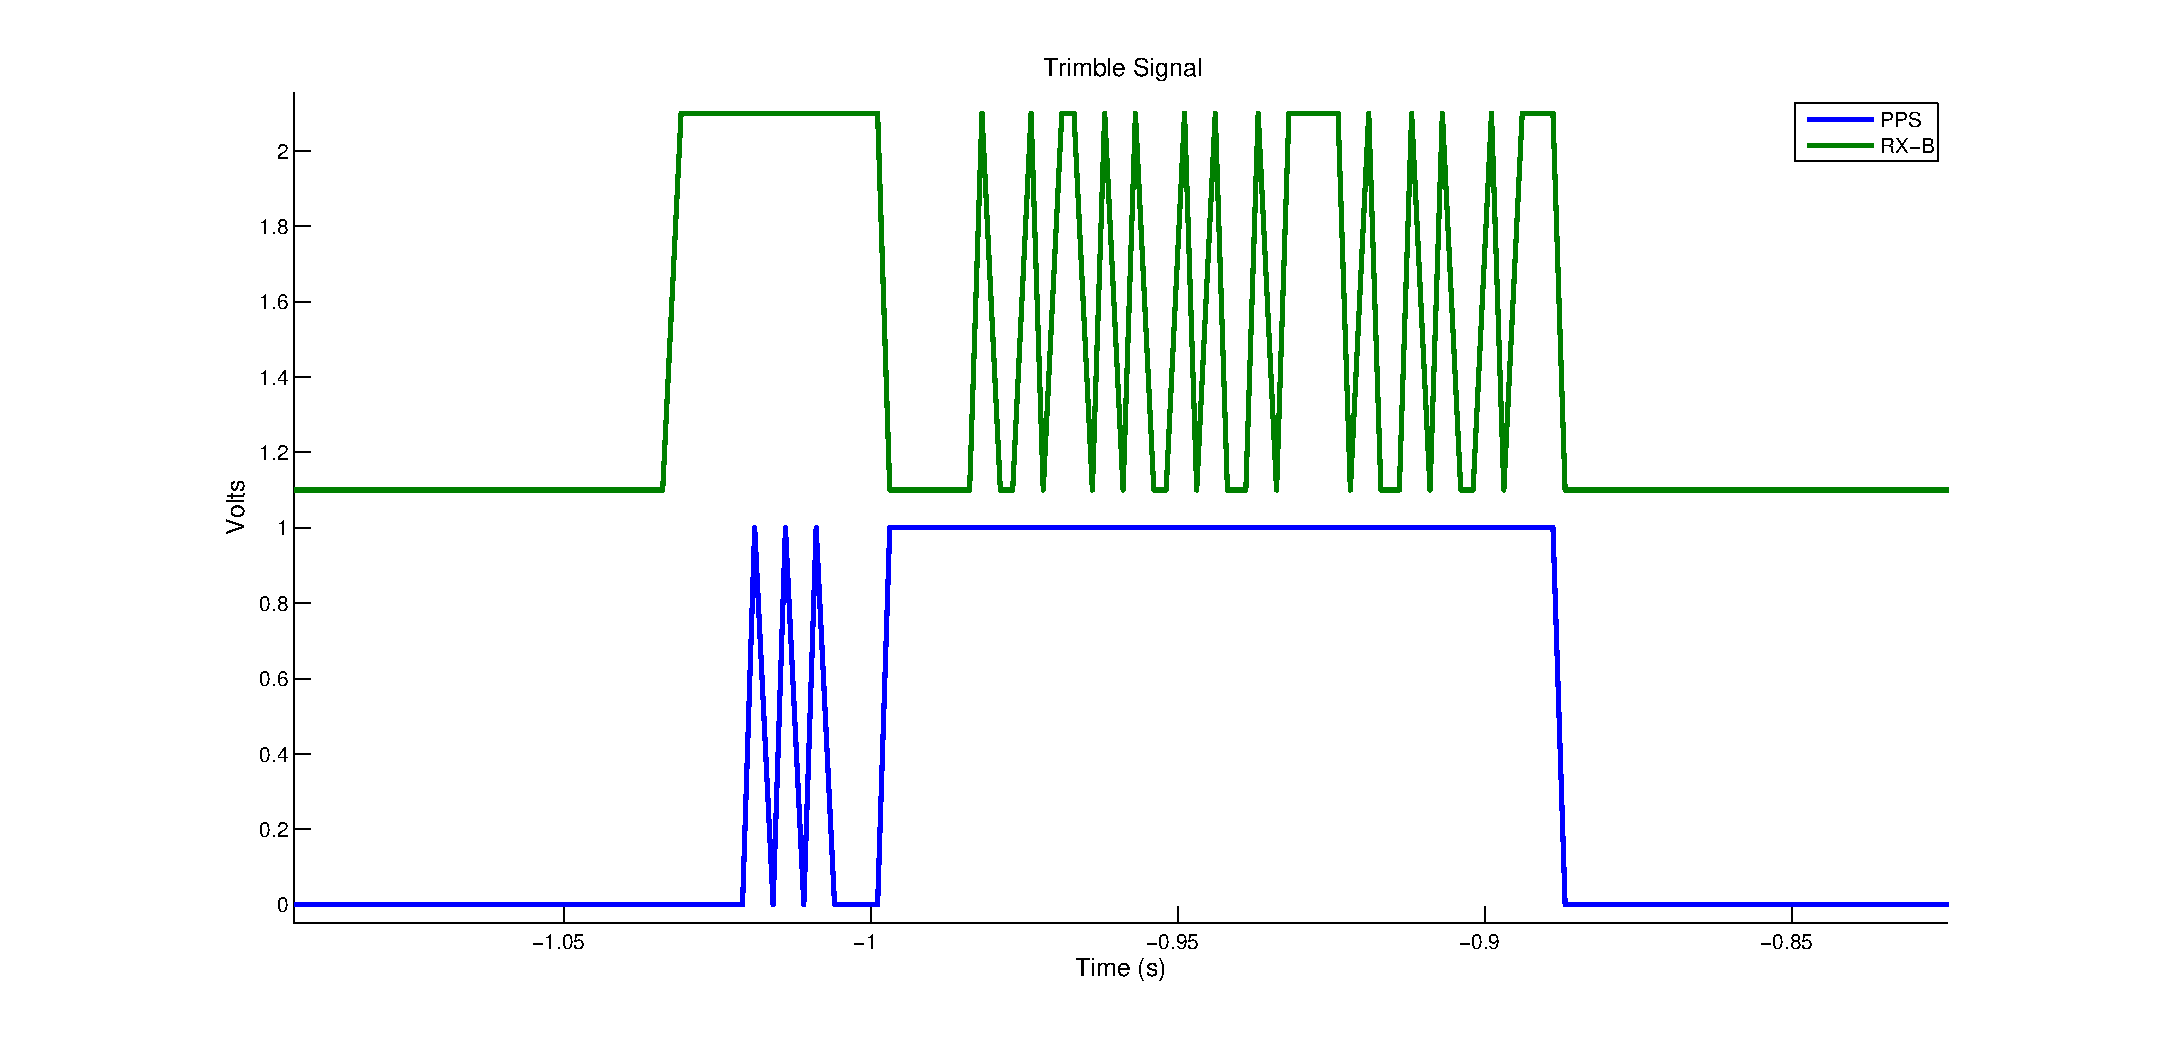
\includegraphics[width = 0.75\linewidth]{Trimble}
\caption{\textit{GPS sentence data and PPS signal recorded with oscilloscope for preliminary analysis.}}
\label{fig:GPS_PPS}
\end{figure}
%\end{landscape}

\section{Power Budget}
\indent After analyzing the power consumption of the individual components of the sensor package, the following power budget was formed (Table
\ref{tab:Power_Budget}). Note that there was a $+10\%$ allocation added to the total power calculated. This was to account for any errors in calculation or
any miscellaneous items that were looked over. 

\begin{table}[H]
\begin{tabular}{|l|l|}
\hline
\textbf{Component}                                          & \textbf{Power Consumption (mW)} \\ \hline
$\mu$ Processor                                      & 1500                   \\ \hline
ADC                                                & 0.66                   \\ \hline
GPS                                                & 132                    \\ \hline
Wireless Transmitter (Anticipated)                 & 800                    \\ \hline
Strain Gauge                                       & 95                     \\ \hline
Accelerometer                                      & 1.4                    \\ \hline
Total                                    & $\approx2530$          \\ \hline
\textbf{Approximate Total Power Consumption +10\%} & \boldmath{$\approx2800$} \\ \hline
\end{tabular}
\caption{\textit{Power budget created based off of the specifications of the components purchased, plus a ten percent buffer.}}
\label{tab:Power_Budget}
\end{table}
% % % % % % % % % CJ


% Data collection------------------------------------------------------------------------------------
\chapter{Data Collection}
\subsection{Camera}
\indent A Contour 1500 version 1.0 was used to record audio video files, in a .MOV format. The I-beam was oriented with the flange facing on the ground, supported by two steel pins. The top flange was struck with a claw hammer at the center of the beam and allowed to resonate until the vibrations had completely dissipated. Next the beam was rotated such that the web was level with the ground. The web was struck with a claw hammer at the center of the beam and allowed to resonate. 

\indent The files were converted to wave (.WAV) audio files for data analysis. The microphone on the camera is assumed to have a flat frequency response. The maximum observable frequency is 2400 Hz, based on Nyquist sampling theorem for a sampling rate of 4800 Hz. MATLAB was used to view a time series of the signal and compute the fast Fourier transform (FFT) of the signals.

Figure \ref{fig:RES_Cam_WebFlange} shows clipping for a very brief period. The signal can be seen decaying very rapidly.

\begin{figure}
\centering
\includegraphics*[width = 0.75\linewidth]{WebFlange.eps}
\caption{\textit{Initial time series data of I-beam excitation test}}
\label{fig:RES_Cam_WebFlange}
\end{figure}

\indent The FFT of the signal, \ref{fig:IbeamFFT} shows some variance between the spectral data of the two signals but both share a common peak at 58.6 Hz proving that regardless of which portion of the beam is struck the entire beam will resonate as a single body rather than different components vibrating independently.  The beam appears to be too rigid during the experiment. A first mode at 58.6 Hz is relatively large compared to the full size bridge with a frequency on the order of 1 Hz. A longer less rigid beam was suggested to lower the frequency. 

\begin{figure}
\centering
\includegraphics*[width = 0.75\linewidth]{Ibeam}
\caption{\textit{FFT for web and flange}}
\label{fig:IbeamFFT}
\end{figure}

\subsection{Piezo Electric Strip}
\indent A DT series piezo electric strip was mounted with 3M double sided foam tape to the inside of the L beam. As the beam flexes a voltage is generated by the sensor and captured as a coma separated value (.CSV) file on a Tektronix oscilloscope. The factory calibration is 10 millivolts per micro strain. 

\indent The cursor tool on the oscilloscope was used to measure the period of one oscillation for a quick measurement of the frequency of the primary mode of the beam. A FFT was performed on a one second clip recorded on the oscilloscope

\begin{figure}[H]
\centering
\includegraphics*[width = 6in]{oscopeTIME.eps}
\caption{\textit{Time-series data for piezo-electric strip testing}}
\label{fig:RES_PEST}
\end{figure}

\indent A peak frequency of 3.05 Hz was recorded using the piezo-electric strip, see Appendix \ref{app:AngleFFT1.jpg}.

\subsection{3g Tri-Axial Accelerometer}
\indent The ADXL330 3g accelerometer was mounted on a breadboard, spring clamped to the center of the beam. The outputs of the three axes were sampled on a National Instruments BNC-2110 DAQ. The beam was deflected and released until no more vibrations were observed. The process was repeated with the accelerometer at 1/3, 1/4, and 1/5 the length of the beam.

\indent Upon initial analysis of the time series, it was observed that the signal did not change regardless of accelerometer placement, Figure \ref{fig:onemode}. All four experiments show the beam vibrating at 2.68 Hz. 

\indent The results from the prior experimental method proved unsuccessful and resulted in changing the method of exciting the beam. In order to excite higher order modes a hammer was used to strike the bean at 1/8, 1/10, 1/16 the length of the beam for the four accelerometer locations. The full time series plot for the 3 strike locations and 4 accelerometer locations can be seen in Appendix \ref{app:RES_3g_T_ALL}. 

\begin{figure}[H]
\centering
\includegraphics*[width = 6in]{onemode.eps}
\caption{\textit{Time series for 3g tri-axial accelerometer data}}
\label{fig:onemode}
\end{figure}

The data from the experiment with 4 accelerometer locations and 3 strike locations produced higher quality data than the previously performed experiments. \ref{fig:clipping}, shows that the accelerometer exceeded the 3g threshold, 2.886 volts in several of the trials. 

\begin{figure}[H]
\centering
\includegraphics*[width = 6in]{clipping}
\caption{\textit{Clipped data from fifth 16 iteration}}
\label{fig:clipping}
\end{figure}

A filter was tested on unclipped data to see if there were any higher frequencies that were being aliased. A low pass filter set to 300Hz was selected because it matched the bandwidth of the accelerometer. Figure \ref{fig:filter} shows the filtered data matches with the raw data. 

\begin{figure}[H]
\centering
\includegraphics*[width = 6in]{filter}
\caption{\textit{300 Hz lowpass filtered}}
\label{fig:filter}
\end{figure}

\indent The Y and Z axis are both in the plane orthogonal to the length of the beam. Although the time series shows that the Y and Z axis do not move in phase, the FFT shows that both channels have the same modes. To reduce the amount of computations in further experiments an analysis of only one channel was performed.

\subsection{6g Tri-Axial Accelerometer}
\indent Figure \ref{fig:DC_AccPlacingIdeal} shows the strike location and accelerometer location to capture the first five idealized modes. By leaving the accelerometer at mid span all the odd modes should show while the even modes will be suppressed because the accelerometer is on a node. 

\begin{figure}[H]
\centering
\includegraphics*[width =6in]{ideal5.jpg}
\caption{\textit{Plot showing the ideal location for mounting the accelerometer in order to capture the first five modes of vibration}}
\label{fig:DC_AccPlacingIdeal}
\end{figure}
\indent The time series recorded to the internal memory on the microprocessor was converted into spectral data using an FFT. Due to hardware limitations of 3 input channels at the time of testing the Y and Z channels of the MMA7361L 6g accelerometer were connected to the external ADC on the BBB, as well as the output of the strain gauge. The X channel was ignored because the beam will not accelerate in the direction of the beam because of the boundary conditions. The Wheatstone bridge was not used because differential inputs were not available. The reference voltage was assumed to be constant at half of the input voltage, generated from the bench top power supply. A 120 $\Omega$ resistor was still used to complete the voltage divider circuit. A time series of the three channels was recorded. 

\chapter{Finite Element Modeling}
\section{Introduction}
\indent A finite element model considers a system and divides it into finite elements and applies material structural properties. The physical response of the structure to an applied loading is added to the initial configuration of the structure. Abaqus is a computer software which calculates approximate finite element solutions for displacements, deformation, stresses, forces, etc. while maintaining force and momentum equilibrium. The state of the model is updated throughout the analysis steps and the effects of the previous step are included in the response of each new step. \\
\indent By completing a finite element model of the simply supported beams approximate modal responses of the beams will indicate the best locations for the sensor package. For the two simply supported beams the modal shapes are trivial, however, the modal response for a complex structure, like the Newport bridge, anticipating modal response is near impossible with hand calculations. \\
\indent Abaqus provides multiple ways to model a particular structure. When modeling the Newport Bridge it will be necessary to use the physical properties, such as length and profile, rather than physical properties, such as moment of inertia, to model quickly. To ensure that Abaqus is calculating moment of inertia as anticipated, analytical solutions can be compared with the results modal frequencies of the Abaqus model. Abaqus allows for two different options of modeling, inputting the moment of inertia or imputing the profile of the element and allowing Abaqus to calculate moment of inertia. \\

\section{Beam Analysis}
\subsection{I Beam Analytical Solution}
\indent For the analysis of the I beam that was assumed to be aluminum 6160, it was modeled in Abaqus and an analytical solution was found to compare. The analytical solution was calculated using Equation \ref{eqn:FEM_Anal}\\
\begin{equation}
F_{n}=\frac{1}{2\pi}\biggl[\frac{n \pi}{L} \biggr]^{2}\sqrt{[\frac{EI}{\rho}} , n=1,2,3\dots\infty
\label{eqn:FEM_Anal}
\end{equation}
\noindent The inputs for the analytical calculations and the Abaqus model are displayed in Table \ref{tab:FEM_inputs}

\begin{table}
    \begin{center}
    \begin{tabular}{|l|l|}
        \hline
        \textbf{Parameter}    & \textbf{Value}     \\ \hline
        Length                & 6.1 m         \\\hline
        Moment of Inertia Ixx & 2.93e-7 m$^4$ \\\hline
        Moment of Inertia Iyy & 1.36e-6 m$^4$ \\\hline
        Modulus of Elasticity & 6x10$^6$GPa      \\\hline
        \end{tabular}
        \caption{\textit{Input parameters for analytical and model solutions.}}
        \label{tab:FEM_inputs}
    \end{center}
\end{table}

\indent The frequencies of the analytical solution and the Abaqus model are very close. This is very important to the progression of this project as Abaqus must be trusted to calculate the moment of inertia within the program. \\
\indent As these frequencies go up above 100 Hz it was anticipated that the sampling frequencies that would be required to properly measure the dynamic response of the beam for the designed sensor package. Analysis was continued with a longer stiffer beam to capture lower frequencies. 

\subsection{L Beam Analysis}
\indent For the analysis of the 6.8 meter L beam the beam was modeled two different ways to confirm that Abaqus program to calculating the moment of inertia properly. The beam was modeled as 6.1 meters long, as the supports were 0.2 meters from either end, with a tri axial restriction boundary condition on one side and a vertical restriction boundary condition on the other side. In the initial model an undefined profile was used and the moment of inertia was imputed. In the second model, a preset profile was used and Abaqus calculated the moment of inertia. The results of those models are as follows (Table \ref{tab:FEM_Abaqus_Comp}):\\

\begin{table}[H]
\begin{center}
    \begin{tabular}{|l| p{3.5cm}| p{3cm}| p{3cm}| p{3cm}|}
    \hline
    \textbf{Mode} & \textbf{Analytical Values} & \textbf{General Profile Abaqus Model Frequency}& \textbf{Input Profile Abaqus Model Frequency} \\\hline
    1    & 3.1 Hz            & 3.1 Hz                             & 3.1 Hz     \\\hline
    2    & 12.4 Hz           & 12.5 Hz                            & 12.4 Hz     \\\hline
    3    & 27.9 Hz           & 27.8 Hz                            & 27.8 Hz     \\\hline
    4    & 49.6 Hz           & 48.8 Hz                            & 48.6 Hz      \\\hline
    5    & 77.5 Hz           & 74.5 Hz                            & 74.4 Hz    \\\hline
    \end{tabular}
    \caption{\textit{Comparison between Abaqus models}}
    \label{tab:FEM_Abaqus_Comp}
\end{center}
\end{table}

\subsection{Results of Experimental Data}
\indent Vibration data for the L beam were collected with a microphone, piezoelectric strip, 3g accelerometer to computer, and 6g accelerometer to our sensor package. Vibration frequencies of the angle beam was captured by mounting an accelerometer to the beam and striking the beam. The 3” x 3” aluminum angle beam of 3/16 thickness was placed open end down, with right angle pointing upward, and struck. Configurations varied for supports, strike locations, and accelerometer placement locations. The first test was done using a piezoelectric strip to detect vibration. The second series of tests was done with a 3g accelerometer (anything above acceleration of 3g is clipped). The third series was done with a 6g accelerometer.
\indent The accelerometer was used to gather vibration data at four different locations. These were at a distance of L/2, L/3, L/4 and L/5 from the angle support, where L is 240” (the length of the supported section of beam).\\
\indent For each accelerometer position, the beam was struck at distance L/8, L/10 and L/16 from the angle support. During the tests using the accelerometers, the beam was struck gently as to minimize or prevent clipping by exceeding accelerometer range of measurement. The results of the best experimental data are shown in Table \ref{tab:Results_Comp}.\\
\begin{table}
\begin{center}
    \begin{tabular}{|l| p{3.5cm}| p{3cm}| p{3cm}| p{3cm}|}
    \hline
    \textbf{Mode} & \textbf{Analytical Values} & \textbf{Values for the generalized profile} & \textbf{Values for the Input profile} & \textbf{Experimental} \\\hline
    1    & 3.1 Hz            & 3.1 Hz                             & 3.1 Hz                       & 3.2 Hz       \\\hline
    2    & 12.4 Hz           & 12.5 Hz                            & 12.4 Hz                      & 12.5 Hz      \\\hline
    3    & 27.9 Hz           & 27.8 Hz                            & 27.8 Hz                      & 27.6 Hz      \\\hline
    4    & 49.6 Hz           & 48.8 Hz                            & 48.6 Hz                      & 48.4 Hz      \\\hline
    5    & 77.5 Hz           & 74.5 Hz                            &                             & 78.5 Hz      \\\hline
    \end{tabular}
    \caption{\textit{Comparison between analytical, model and experimental results}}
    \label{tab:Results_Comp}
\end{center}
\end{table}

\section{Limitations of Abaqus Model}
\indent Although finite element analysis has enables engineers and scientists gain an understanding of a structure’s behavior and dynamic response, it is very important to know the limitations of finite element modeling. Abaqus must be used as a research tool and not considered the basis of design. Mesh resolution will change the dynamic response and accuracy of the solution. \\
\indent When modeling within Abaqus and indicating a particular profile, the preset profiles that are available do not match perfectly with the profiles that were used in experiments. As the frequencies resultant for the two different modeling techniques were not considerable different, the error acquired within the dissimilarity cannot be significant and thus negligible by evaluations. \\

\chapter{Future Development}
%\section{Finite Element Model}
\section{Power System}
%\subsection{Wireless Communication}
\subsection{Power System: Energy Scavenging}
% % % % % %MIKE
\indent The design of a sensor package with multiple instruments requires careful planning in order for each piece to work properly and accurately. Creating a package that continuously takes measurements and wirelessly transmits this data raises the question of how to power the system. One solution to this issue of power is the use of a battery that is strong enough to run all components of the package. This system is designed to monitor a structure for a number of years, making energy storage imperative.\\
\indent In order to prove that batteries alone are not sufficient to power the instrumentation package for a duration of 10 years, preliminary calculations were carried out for a heavy duty Lead-Acid battery. It was determined that over 1000 batteries would be necessary to provide energy for a period ten years. The reason for carrying out these preliminary calculations was to prove without question, that the instrumentation package would have to be powered by the scavenging and storage of energy. \\
\indent Energy can be scavenged in a number of ways, the more popular methods use abundant resources such as solar and wind energy. In the first phase of this project, the theoretical average power per day was calculated and analyzed based on NOAA data. In the second phase of this project, the purchase and design of a solar panel, wind turbine, and rechargeable battery system will be field tested. Ideally, this hybrid energy storage system will ensure for the long term health monitoring of a structure. \\
\indent The FEM analyses were verified with analytical solutions and experimental data, confirming the natural frequencies for the I-beam and the angle beam. This has proven that an Abaqus model of the Claiborne Pell Newport Bridge is feasible to be created in phase two of the project. 

\subsubsection{Solar Power}
\indent The National Oceanic and Atmospheric Administration (NOAA) is a scientific agency that is a part of the U.S. department of commerce. Through the Earth System Research Laboratory, NOAA offers datasets for various climate properties such as humidity, temperature, cloud coverage and solar radiation. Data for the downward short wave radiation flux, (DSWRF) is available for download for the past 65 years \cite{Kistler01thencepncar}. These files can be imported into MATLAB and refined for the values relevant to a desired location based on its respective longitude and latitude as the data is recorded for all locations around the world. To obtain more accurate data, measurements for the daily mean taken every six hours were uploaded, rather than using data collected once every day. A plot of the four times daily mean power versus the average daily power for the year 2010 are seen in Figure \ref{fig:SOLAR_avg_power} below. By using solar data for the past 6 years, the yearly trend for the change of season becomes clear and is more accurate than using one year of data.\\

\begin{figure}[H]
\centering
\includegraphics*[width = 6in]{Mean_Power_2010}
\caption{\textit{Plot of average daily power for Newport, Rhode Island}}
\label{fig:SOLAR_avg_power}
\end{figure}
\indent The theoretical maximum daily power is around 300 Watts per square meter, where as the minimum average power dips below 100 Watts per square meter. It is important to note that these values will decrease dramatically in the second phase of the project taking into account the efficiency and surface area of the desired solar panel. \\
\indent From the daily average solar flux taken every six hours, MATLAB plots the solar flux in units of Watts per square meter versus time in units of days. By taking the mean of the four data points per day, an array of 365 data points for average power per day is obtained. Cumulatively integrating the daily average power yields the average energy per day for a given year, solar energy is in units of Watt hours per square meter. Ultimately, the total energy averaged over all six years gives a more confident set of values. \\
\indent Calculating the standard deviation for average daily energy for January through December of all six years will allow for a greater level of confidence. By finding the first and second standard deviation above and below the mean daily energy, the percent confidence increases. In other words, using the first and second standard deviation results in a $68.2\%$ and $95\%$ confidence, respectively. This statistical analysis is illustrated in Figure \ref{fig:SOLAR_Avg6}, where the mean daily energy as well as the first and second standard deviation are plotted. Various markers for each individual data point over all six years are identified in the legend.\\

\begin{figure}[H]
\centering
\includegraphics[width = \linewidth]{Avg_Energy_6Years.eps}
\caption{\textit{Plot displaying the average energy for 6 years.}}
\label{fig:SOLAR_Avg6}
\end{figure}

\indent To ensure that the sensor package has access to ample power, an analysis of the worst-case scenario will be carried out. This is a scenario where there are multiple days in a row with poor sun coverage as opposed to a single day with complete overcast. To better visualize the trend of a year, the mean daily energy for six years was passed through a 7 point moving average filter. This filter takes into account three days before and three days after the data point and averages them. Essentially this produces a smoother curve as seen in Figure \ref{fig:SOLAR_Move_Avg} \\

\begin{figure}[H]
\centering
\includegraphics[width = \textwidth]{SevenDay_Moving_Average_Filter.eps}
\caption{\textit{The 6 years of data was averaged and then smoothed using a 7 day moving average filter.}}
\label{fig:SOLAR_Move_Avg}
\end{figure}
% % % % % % %PAT
\subsubsection{Wind Power}
\indent The site of the Newport Bridge is a suitable location for a wind turbine because the bridge is high off the ground and there are no sounding objects to block the wind. The process of harvesting energy from the wind is simple; wind turns a generator to create electricity. The electricity is then stored in batteries. In addition to the wind turbine a solar panel will be installed to supplement power generation. Due to cost and space limitations, the minimum quantity of batteries required to keep the sensor package running will be used. The sensor package will require a continuous power source in order to collect data. The goal is to collect five years of data from the sensor package. \\   
\indent A NOAA Station  (National Oceanic and Atmospheric Administration) located about 500 meters north of the bridge in Newport, RI collects data continuously every 6 minutes, corresponding to about 87,000 data points a year. The anemometer (wind speed gauge) is approximately 6.4 meters off the ground. \\
\indent For the wind speed to be accurate at the height of where the turbine would be placed on the bridge, the wind data has to be reconfigured. This is done with the wind profile power law: 

\begin{equation}
U_{2} = U_{1}(\frac{Z_{2}}{Z_{1}})^\alpha
\label{eqn:WIND_Power_Law}
\end{equation}
Where $U_{2}$ the wind is speed at height $Z_{2}$, $U_{1}$ and is the wind speed at height $Z_{1}$. $Z_{2}$ is the computed height and is the reference height. is the power law exponent. The power law exponent is a function of the local climatology, topography, surface roughness, environmental conditions, meteorological lapse rate, and weather stability \cite{Zekai}. This makes the wind profile to be logarithmic and not linear. Studies have shown that the power law exponent to be .14 or 1/7 for most sites. The wind data from NOAA, Figure \ref{fig:WIND_6.4}, was put into MATLAB and the wind data for the corresponding height of 50 meters, Figure \ref{fig:WIND_50}, was calculated. The average wind speed at the NOAA station is $4.38 (m/s)$ and the average speed at the corresponding height of 50 meter was $5.83(m/s)$.

\begin{figure}[H]
\centering
\includegraphics*[width = 6in]{WIND_Data_6}
\caption{\textit{Time series for wind data collected in 2012 at 6.4 meters}}
\label{fig:WIND_6.4}
\end{figure}

\begin{figure}[H]
\centering
\includegraphics*[width = 6in]{WIND_Data_50}
\caption{\textit{Time series for wind data collected in 2012 at 10 meters}}
\label{fig:WIND_50}
\end{figure}

\indent The computed wind data was then analyzed and a probability density graph of the wind speed what created in MATLAB. The probability density graph, figure 3, shows the probability of each wind speed.

\begin{figure}[H]
\centering
\includegraphics*[width = 6in]{WIND_PDF}
\caption{\textit{Probability Density Function of computed data}}
\label{fig:WIND_PDF}
\end{figure}

\indent The probability density graph gives a more accurate calculation of the power output. This is because the equation for power is:

\begin{equation}
Power = \frac{A_{S} \times A_{D} \times E \times V^{3}}{2}
\end{equation}

\indent Where $A_{S}$ is the swept area of the turbine blade, $A_{D}$ is the air density and $E$ is the efficiency of the turbine. ($0.5 \times V^{3}$) is velocity participating in a calculation of Kinetic Energy to produce the mass of air on the turbine \cite{arcGIS:2013}. Since Velocity is cubed in this equation, doubling the wind speed would increase the power output by eight. This is why a probability density graph is better than just a yearly average. Also if the radius of the turbine is doubled the power output would increase by four. \\
\indent The wind turbine that is under consideration for this package has a radius of .127 meters. This gives a swept area of approximately .051 m2. The maximum efficiency of any wind turbine can only be $59\%$ but this wind turbine is closer to $40\%$ \cite{Windpower}\\
\indent With the power equation, turbine efficiency, and the probability density graph, an approximation can be made about the power output from the NOAA data. The annual output with this turbine at this location was calculated to be around 37,000 Watt hours. Without knowing exactly what instruments and draw that the sensor package is going to have, there is no definite answer that the purposed turbine will be able to power this package by itself. 



\chapter{Conclusions}
\indent Over the course of phase one of this project a prototype of the sensor package that will be used in phase two of the project. The components purchased were verified to function as a system for this package. Development must be done on wireless transmission of data, time-synchronization of data and energy scavenging. It is anticipated that the final sensor package will have a custom PCB designed and fabricated to localize the microprocessor, ADC, accelerometer and GPS to one board.\\
\indent 


\appendix
\chapter{Piezo-Electric Frequency Spectrum}
\begin{figure}[h]
\centering
\includegraphics*[width = 6in]{AngleFFT1.eps}
\caption{\textit{FFT from Piezo Electric strip}}
\label{app:AngleFFT1}
\end{figure}

%Oscope FFT
%\begin{figure}[h]
%\centering
%\includegraphics*[width = 6in]{AngleFFT1}
%\caption{\textit{FFT from Piezo Electric strip}}
%\label{app:AngleFFT1}
%\end{figure}

\chapter{Three Strikes at Four Locations}
\begin{figure}[h]
\centering
\includegraphics*[width = \linewidth]{allplots.eps}
\caption{\textit{Time series for 3g tri-axial accelerometer data}}
\label{app:RES_3g_T_ALL}
\end{figure}

\chapter{Odd Modes}
\begin{figure}[h]
\centering
\includegraphics*[width = 6in]{OddModes}
\caption{\textit{Odd Modes}}
\label{app:Odd Modes}
\end{figure}

\chapter{Even Modes}
\begin{figure}[h]
\centering
\includegraphics*[width = 6in]{EvenModes}
\caption{\textit{Even Modes}}
\label{app:Even Modes}
\end{figure}



\bibliographystyle{plain}
\bibliography{KIRBY_ADC,KIRBY_GPS,McINTOSH_STRAIN,WILEY_ACCELEROMETER,BLUM_WIND,REGAN_SOLAR,PAUL_FEM}

\end{document}